\documentclass{article}
% ----- Preamble
\usepackage[utf8]{inputenc} % police encodee en latin1=iso8859-1=Windows Latin 1 %
\usepackage[french]{babel} % police fr %
\usepackage{hyperref} % pour les references %
\usepackage{amsmath} % pour les formules de maths %
\usepackage{amssymb} % pour les symboles maths %
\usepackage{amsthm} % pour la mise en forme des theoremes %
\usepackage{aeguill} % pour les guillemets et accents francais %
\usepackage{listings} % pour les listings de code %
\usepackage{helvet} % police helvetica %
\usepackage{graphicx}
\usepackage{centernot}
\usepackage{dsfont}
\usepackage{subcaption}
\usepackage{caption}
% modification des dimensions de la page et de son centrage %
\topmargin 0.0cm
\oddsidemargin 0.1cm
\textwidth 16cm 
\textheight 22cm
\footskip 0.0cm

\title{Traitement d'Image et du Signal - TP5}
\author{Laurent Cetinsoy, Karim Kouki, Aris Tritas }
\date{\today}

\begin{document}
\maketitle

\section{Egalisation d'histogramme}
L'objectif de l'égalisation d'histogramme est de rehausser le contraste d'une image. Les libraires standard de Matlab et Octave implémentent la fonction \textsf{histeq}. Ci-dessous un exemple d'image dont l'histogramme a été égalisé par cette fonction. Les couleurs sombres sont clairement exaggérées.

\begin{figure}[h]
	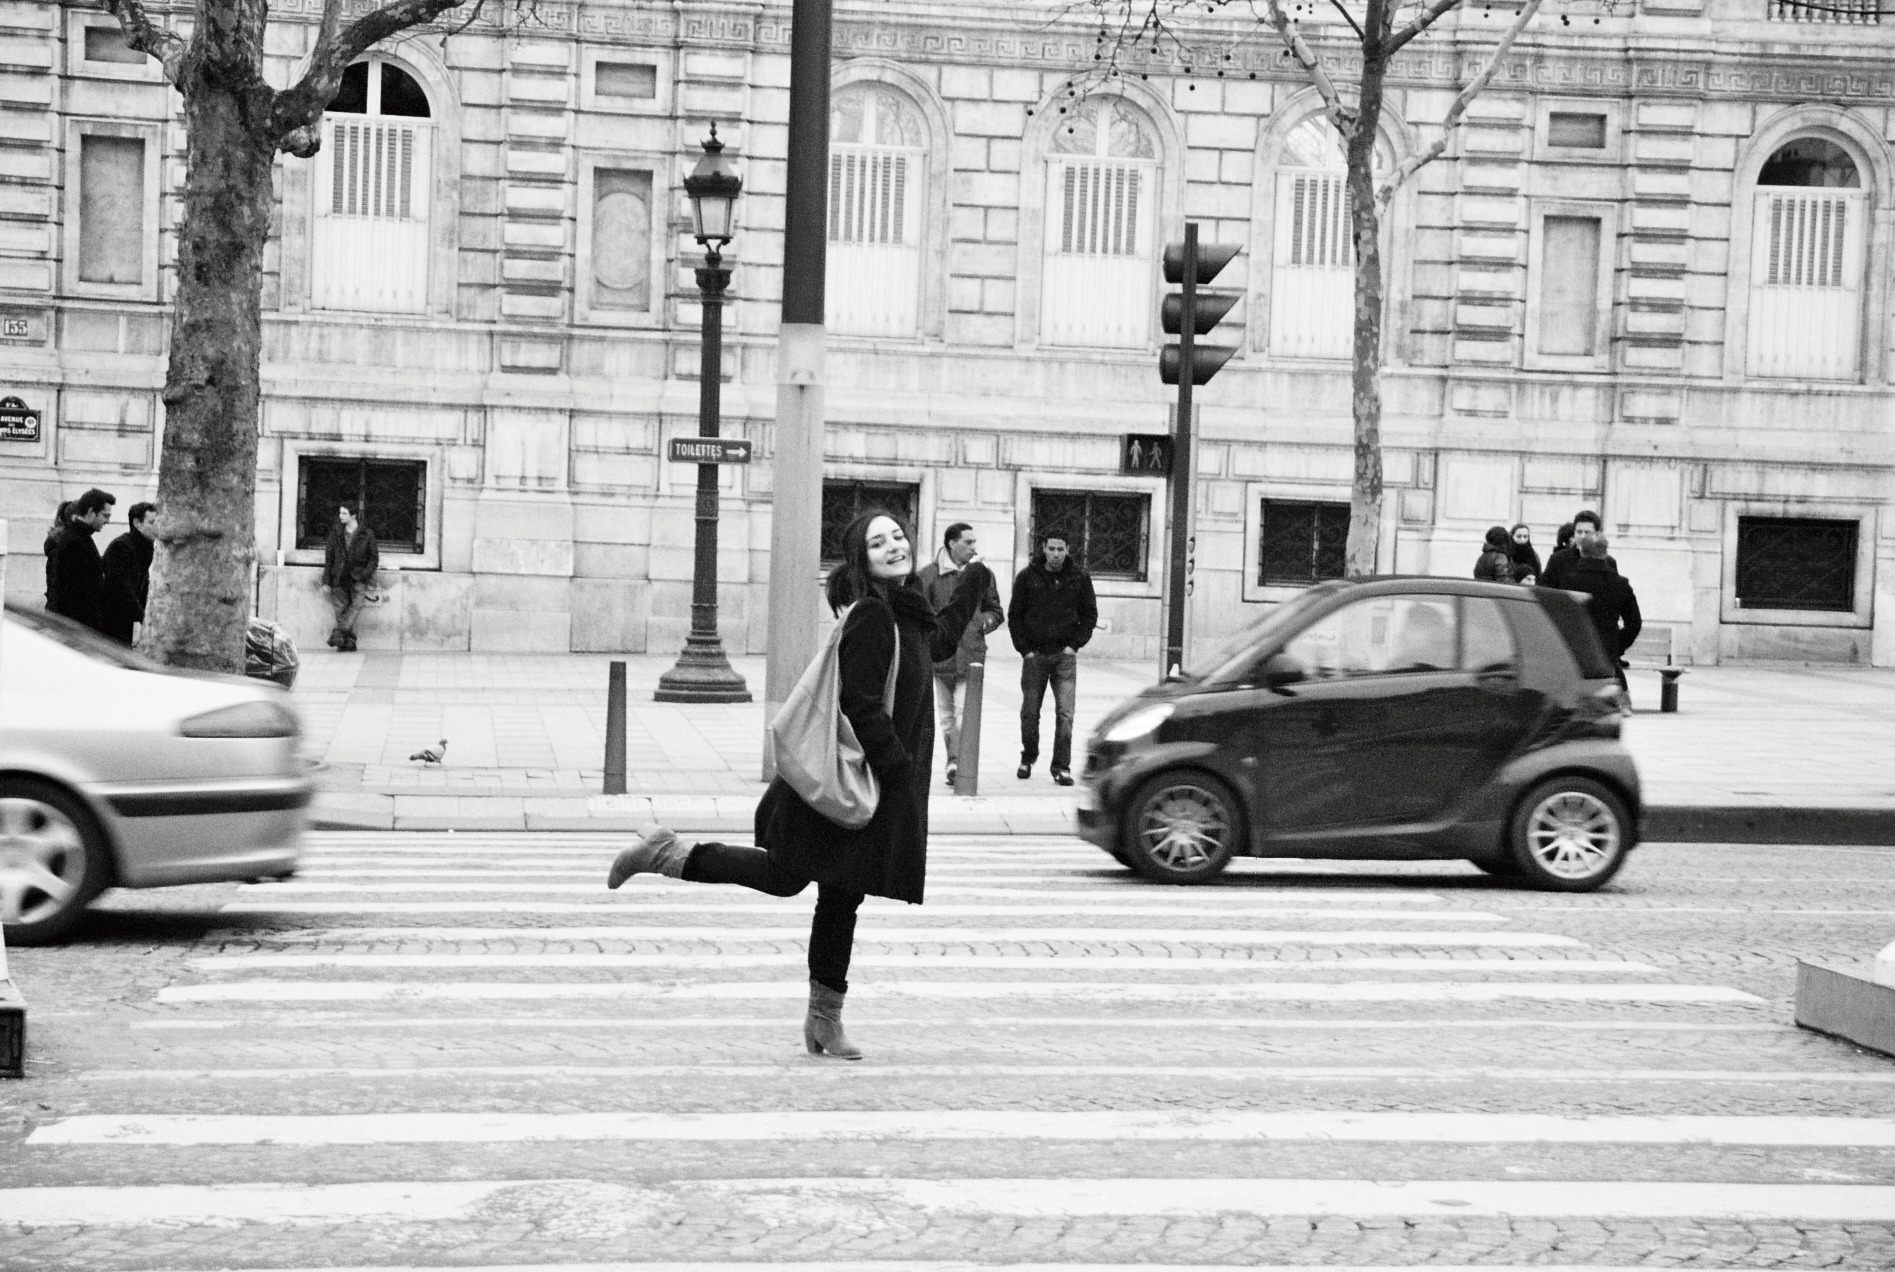
\includegraphics[width=0.5\textwidth]{P11.jpg}
	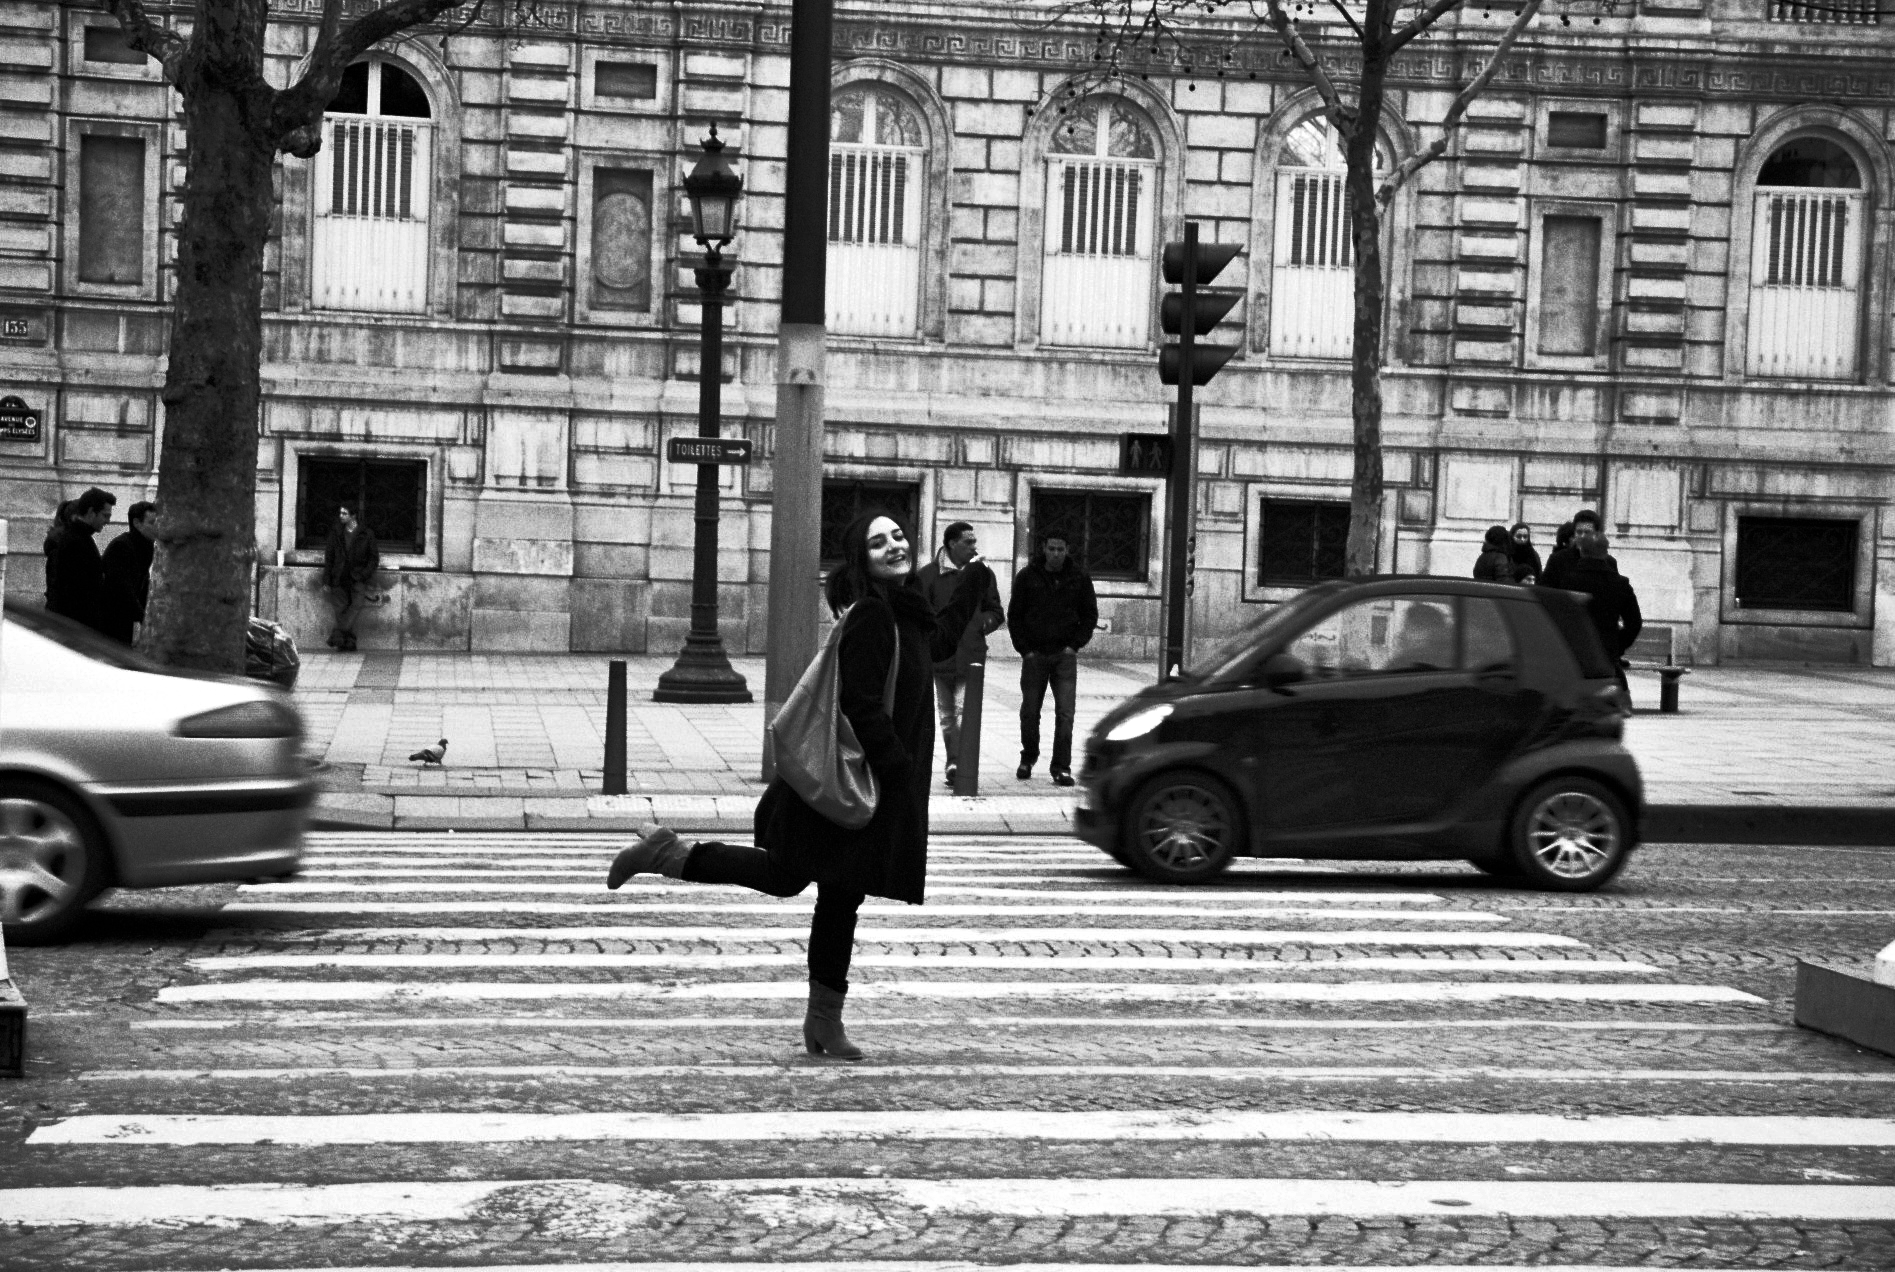
\includegraphics[width=0.5\textwidth]{P11eq.png}
	\newline
	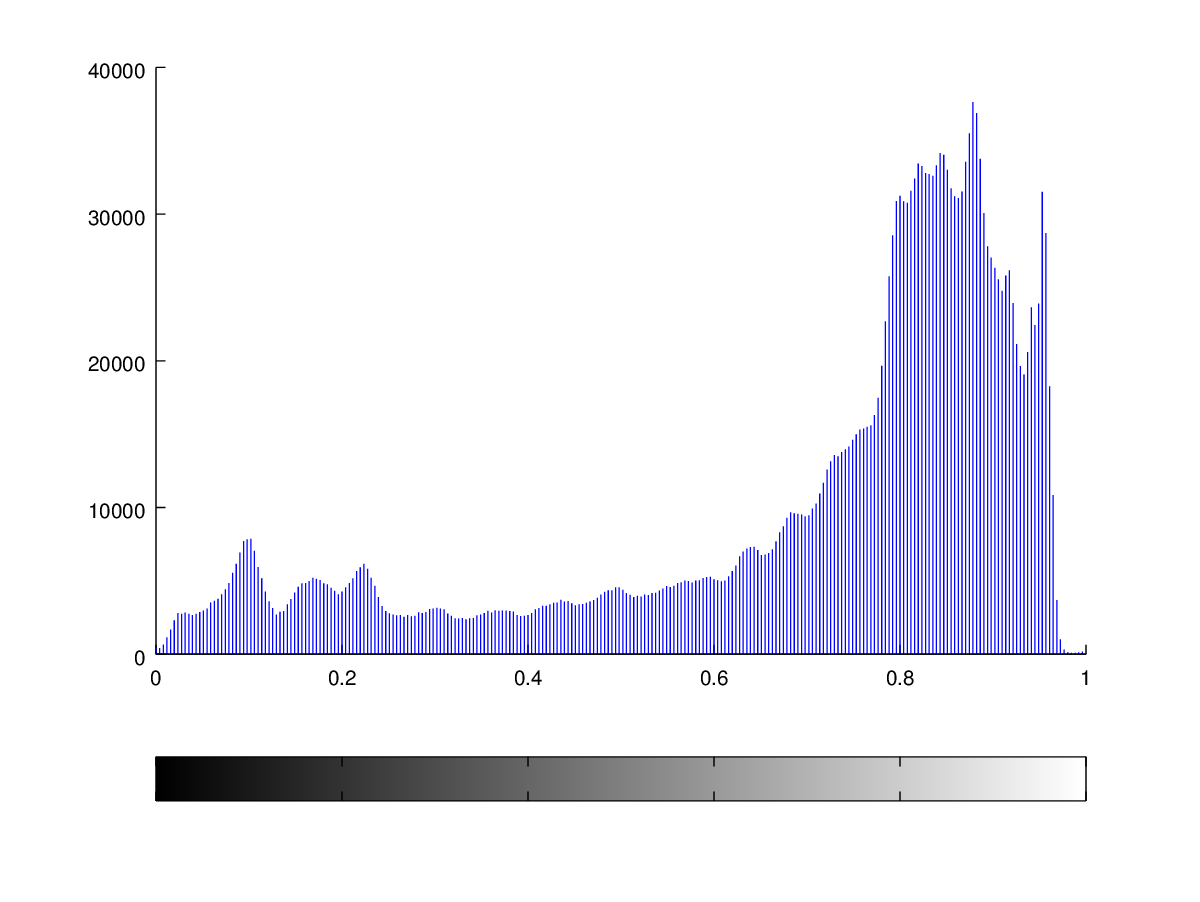
\includegraphics[width=0.5\textwidth]{hist_p11.png}
	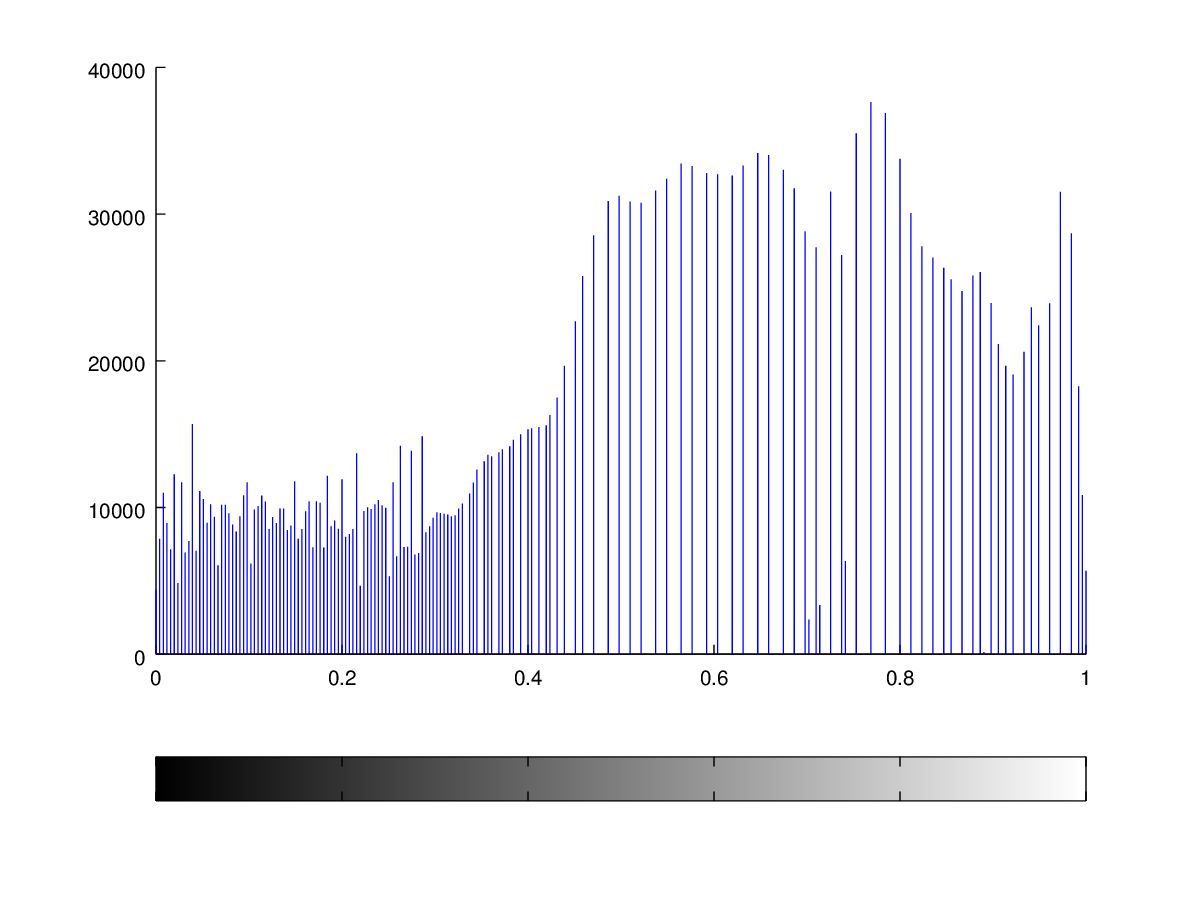
\includegraphics[width=0.5\textwidth]{hist_p11eq.png}
  \caption{A gauche l'image originale et l'histogramme correspondant. A droite l'image dont l'histogramme a été égalisé. }
\end{figure}

\begin{figure}[h]
  \caption{}
\end{figure}


\section{Méthode du Midway}
La méthode du Midway consiste à faire la moyenne harmonique de deux images en spécifiant pour chacune l'histogramme moyen des deux. Ici un premier exemple en niveaux de gris, et un autre en couleur.

\begin{figure}[h]
	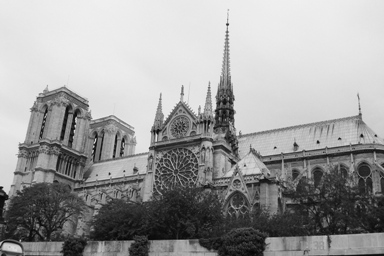
\includegraphics[width=0.33\textwidth]{NotreDame1.png}
	
\includegraphics[width=0.33\textwidth]{NotreDame2.png}
	
\includegraphics[width=0.33\textwidth]{NotreDame1M.png}
  \caption{De gauche à droite: Notre-Dame sur-exposée, sous-exposée, et midway}
\end{figure}

\begin{figure}[h]
	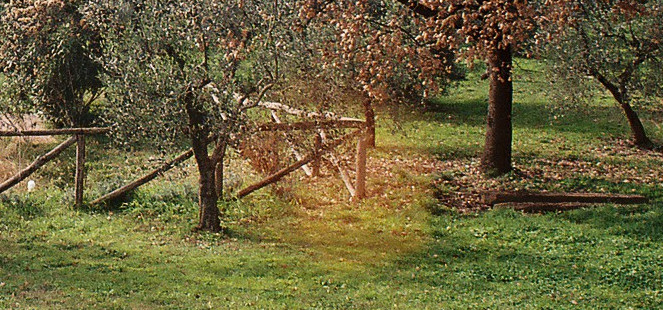
\includegraphics[width=0.33\textwidth]{P1c.jpg}
	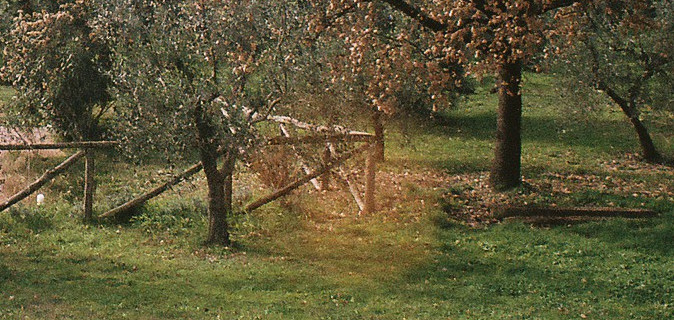
\includegraphics[width=0.33\textwidth]{P2c.jpg}
	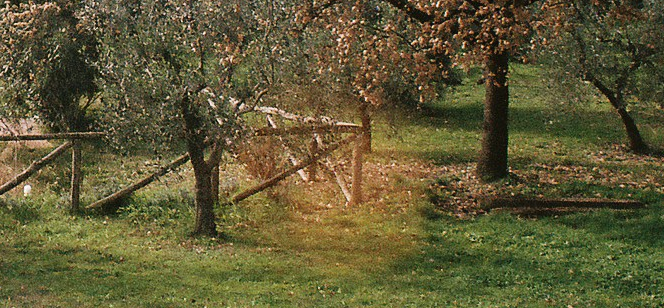
\includegraphics[width=0.33\textwidth]{P1Mc.png}
  \caption{De gauche à droite: patch sur-exposé, sous-exposé et midway}
\end{figure}

\section{Images de bruit gaussien}
Chacune des images ci-dessous ont des pixels distribués selon la loi normale: $I \sim \mathcal{N}(\frac{1}{2}, \sigma^2)$

\begin{figure}[h]
	
\includegraphics[width=0.33\textwidth]{noise001.png}
	
\includegraphics[width=0.33\textwidth]{noise01.png}
	
\includegraphics[width=0.33\textwidth]{noise10.png}
  \caption{De gauche à droite $\sigma^2 = \frac{1}{100}, \frac{1}{10}, 1$}
\end{figure}
\newpage
\section{Filtre bilatéral}
L'objectif est d'implémenter une forme simple du filtre bilatéral.
\subsection{Implémentation}
\subsubsection*{Q1}
$$w \in \mathbb{N}^+ \;, \; y \in \Omega(p) \rightarrow (y-p) \in {[{-w}, w]}^2$$
\subsubsection*{Q2}
Soit $\Omega(p) \ni y \rightarrow f_s(\parallel y-p \parallel_{\ell^2})$. 
D'après la question précédente: $ 0 \leq \parallel y-p \parallel_{\ell^2} \leq 2 w^2 $

Or $f_s$ est décroissante sur $\mathbb{R}_+$, donc: $$\exp(-(\frac{w}{\sigma_s})^2) \leq f_s(\parallel y-p \parallel_{\ell^2}) \leq 0 $$

\subsubsection*{Q3} D'après l'équation 3, nous avons besoin des points du sous-ensemble ci-dessous pour calculer $u_\text{denoised}(p)$ avec p fixé: 

$$\big \{ \: u(y_1, y_2) \;|\; y_1 \in {[p_1 - w, p_1 + w]}, \; y_2 \in {[p_2 - w, p_2 + w]}\: \big \}  $$

\textbf{Remarque: } Il s'agit d'une fenêtre carrée de taille fixe autour du pixel d'intérêt.
\subsubsection*{Q4}
Les conditions que les indices $p_1$ et $p_2$ doivent satisfaire sont:
 $$p_i + w < N \;\text{et}\; p_i - w > 0 \;,\; i \in \{1, 2\} \rightarrow p_1, p_2 \in {[w, N-w]}$$
\subsubsection*{Q5}
On pose les changements de variable: $i_1 = y_1 - p_1 + w + 1$ et $i_2 = y_2 - p_2 + w + 1$

Après re-indexation, l'équation (3) s'écrit:
\begin{equation*}\begin{split}
u_\text{denoised}(p_1, p_2) = \frac{1}{C} \displaystyle\sum_{i_1 = 1}^{2w + 1}
\displaystyle\sum_{i_2 = 1}^{2w + 1} & u(i_1+p_1 - w - 1, i_2 + p_2 - w - 1) \\
& \exp{ \big ( - \frac{(i_1 - w - 1)^2 + (i_2 -w -1)^2 }{2\sigma_s^2} \big )} \\
& \exp{ \big ( - \frac{[u(i_1 + p_1 - w - 1, i_2 + p_2 - w - 1) - u(p_1, p_2)]^2}{2\sigma_i^2} \big )}
\end{split}\end{equation*}

\subsubsection*{Q6}
Ré-écrivons la formule précédente avec les fonctions $S$ et $\tilde{u}$ données:
\begin{equation*}\begin{split}
u_\text{denoised}(p_1, p_2) = \frac{1}{C} \displaystyle\sum_{i_1 = 1}^{2w + 1}
\displaystyle\sum_{i_2 = 1}^{2w + 1} & \tilde{u}(i_1, i_2) S(i_1,i_2) \exp{ \big ( - \frac{[\tilde{u}(i_1, i_2) - u(p_1, p_2)]^2}{2\sigma_i^2} \big )}
\end{split}\end{equation*}

\subsubsection*{Q7}
La constante de normalisation s'écrit de même:
\begin{equation*}\begin{split}
C = \displaystyle\sum_{i_1 = 1}^{2w + 1}
\displaystyle\sum_{i_2 = 1}^{2w + 1} S(i_1,i_2) \exp{ \big ( - \frac{[\tilde{u}(i_1, i_2) - u(p_1, p_2)]^2}{2\sigma_i^2} \big )}
\end{split}\end{equation*}
\subsubsection*{Q8}
D'après ce qui a été dit précédemment, trois matrices seront nécessaires pour implémenter le filtre:
\begin{itemize}
\item une matrice de la taille de l'image pour conserver les résultats de $u_denoised(p)$ durant le parcours de l'image
\item une matrice de taille $w \times w$ à valeurs constantes pour stocker les valeurs du kernel spatial
\item une matrice de taille $w \times w$ à valeurs variables pour stocker les valeurs du kernel d'intensité
\end{itemize}
\subsection{Analyse}

\subsubsection*{Q10. $\sigma_i \rightarrow + \infty $}
On tend à uniformiser la valeur de $p$ sur les intensités voisines. L'on observe par exemple un ``aplatissement'' des tâches spectrales, c'est-à-dire une atténuation de celles-ci sur leur bord.

\subsubsection*{Q11. $\sigma_i \rightarrow 0 $}
Techniquement, le kernel spatial est le seul a être 	pris en compte. En pratique, l'image originale reste inchangée.

\subsubsection*{Q12. $\sigma_s \rightarrow + \infty $}
On tend à uniformiser sur les valeurs des couleurs voisines (ce qui rappelle une convolution gaussienne).

\subsubsection*{Q13. $\sigma_s \rightarrow 0 $}
Le kernel d'intensité est seul pris en compte. De même, en pratique, l'image originale reste inchangée.

\begin{figure}
    \centering
    \begin{subfigure}[b]{0.3\textwidth}
        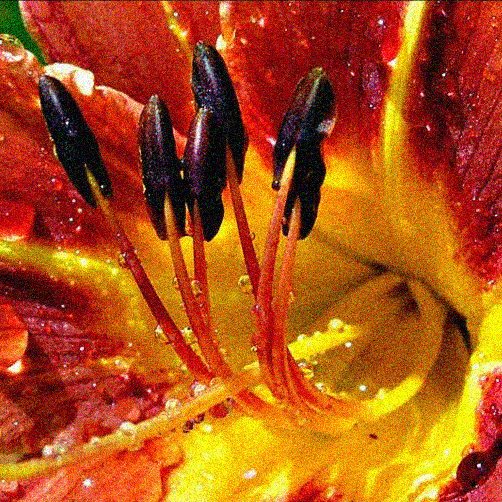
\includegraphics[width=\textwidth]{flowers_noisy.png}
        \caption{Image bruitée, $\sigma=0.1$}
    \end{subfigure}
    \begin{subfigure}[b]{0.3\textwidth}
        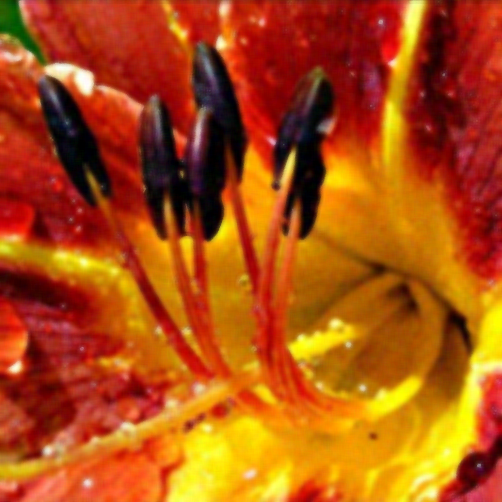
\includegraphics[width=\textwidth]{bilateral10_1.png}
        \caption{$\sigma_s = 10$}
    \end{subfigure}
    \begin{subfigure}[b]{0.3\textwidth}
        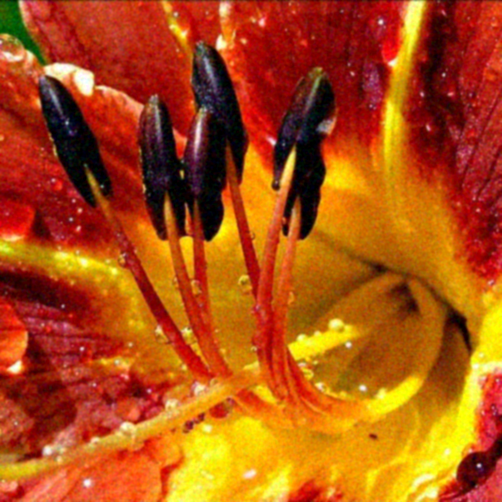
\includegraphics[width=\textwidth]{bilateral1_10.png}
        \caption{$\sigma_i = 10$}
    \end{subfigure}
    \caption{Effet de filtres bilatéraux avec de grands paramètres de kernels.}
\end{figure}
\newpage
\subsection*{Résultats}
Pour une autre image, l'histogramme de l'image résultant du filtrage bilatéral exhibe nettement un lissage de la partie sombre de l'image.
\begin{figure}[ht]
	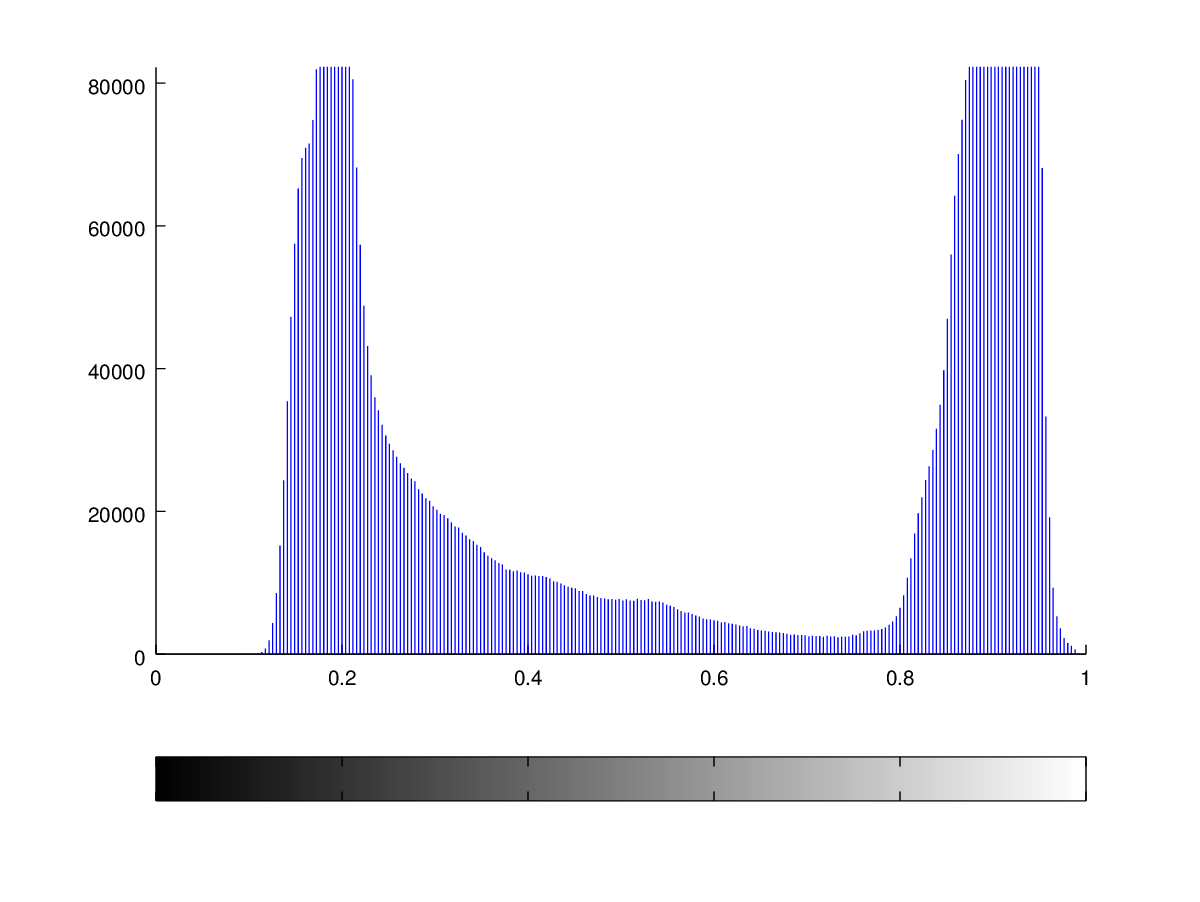
\includegraphics[width=0.5\textwidth]{hist_orig.png}
	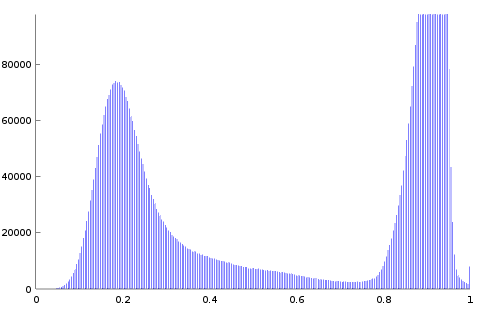
\includegraphics[width=0.5\textwidth]{hist_eq.png}
  \caption{A gauche l'histogramme de l'image originale et à droite l'histogramme après avoir appliqué un filtre bilatéral avec $w=3, \sigma_i = \sigma_s = 1$ }
\end{figure}

\section{Transformée en cosinus discet et zoom par zéro padding}
La transformée en cosinus discret implicite se fait en répliquant une image par symmétrie miroir, elle est ainsi quadruplée. Ci-dessous l'on compare cette méthode et un zéro padding simple sur un patch de l'image finale. L'on constate bien que les raies produites par le zéro padding (oscillations) disparaissent par la périodisation implicite de la TCD.

\begin{figure}[h]
	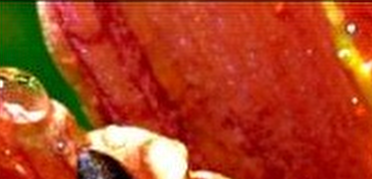
\includegraphics[width=0.50\textwidth]{flowersZerPad.png}
	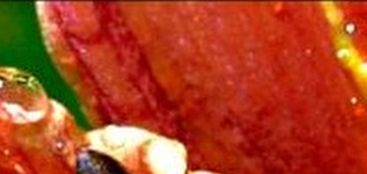
\includegraphics[width=0.50\textwidth]{flowersTCD.png}
  \caption{A gauche l'image est zéro paddée et à droite la TCD implicite a été appliquée}
\end{figure}
\end{document}